\chapter{Logistična regresija}
\label{ch:logisticna-regresija}

Logistična regresija je ena najpreprostejših metod strojnega učenja. \marginnote{Logistična regresija je v resnici klasifikacijska in ne regresivna metoda. Regresija se imenuje zgolj zato, ker je metodološko podobna linearni regresiji.}Deluje s številskimi vrednostmi in je odlična za modeliranje naših genov. V našem delotoku naivnega Bayesa preprosto zamenjamo z gradnikom \widget{Logistic Regression}.

\begin{figure}[h]
    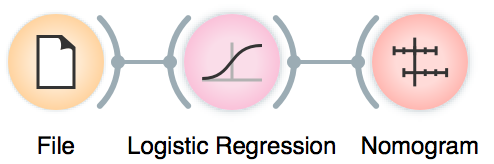
\includegraphics[width=0.6\linewidth]{workflow.png}
    \caption{$\;$}
\end{figure}

V nomogramu so naše vrednosti enakomerno razporejene. To naredi nomogram bolj pregleden, kot je bil prej z naivnim Bayesom. Ena spremenljivka, spo-mid, izstopa: očitno je za napovedni model dvakrat bolj pomembna kot naslednja najpomembnejša spremenljivka. Dolžina lestvice je namreč odvisna od pomembnosti spremenljivke.

\begin{wrapfigure}{o}{1.0\textwidth}
    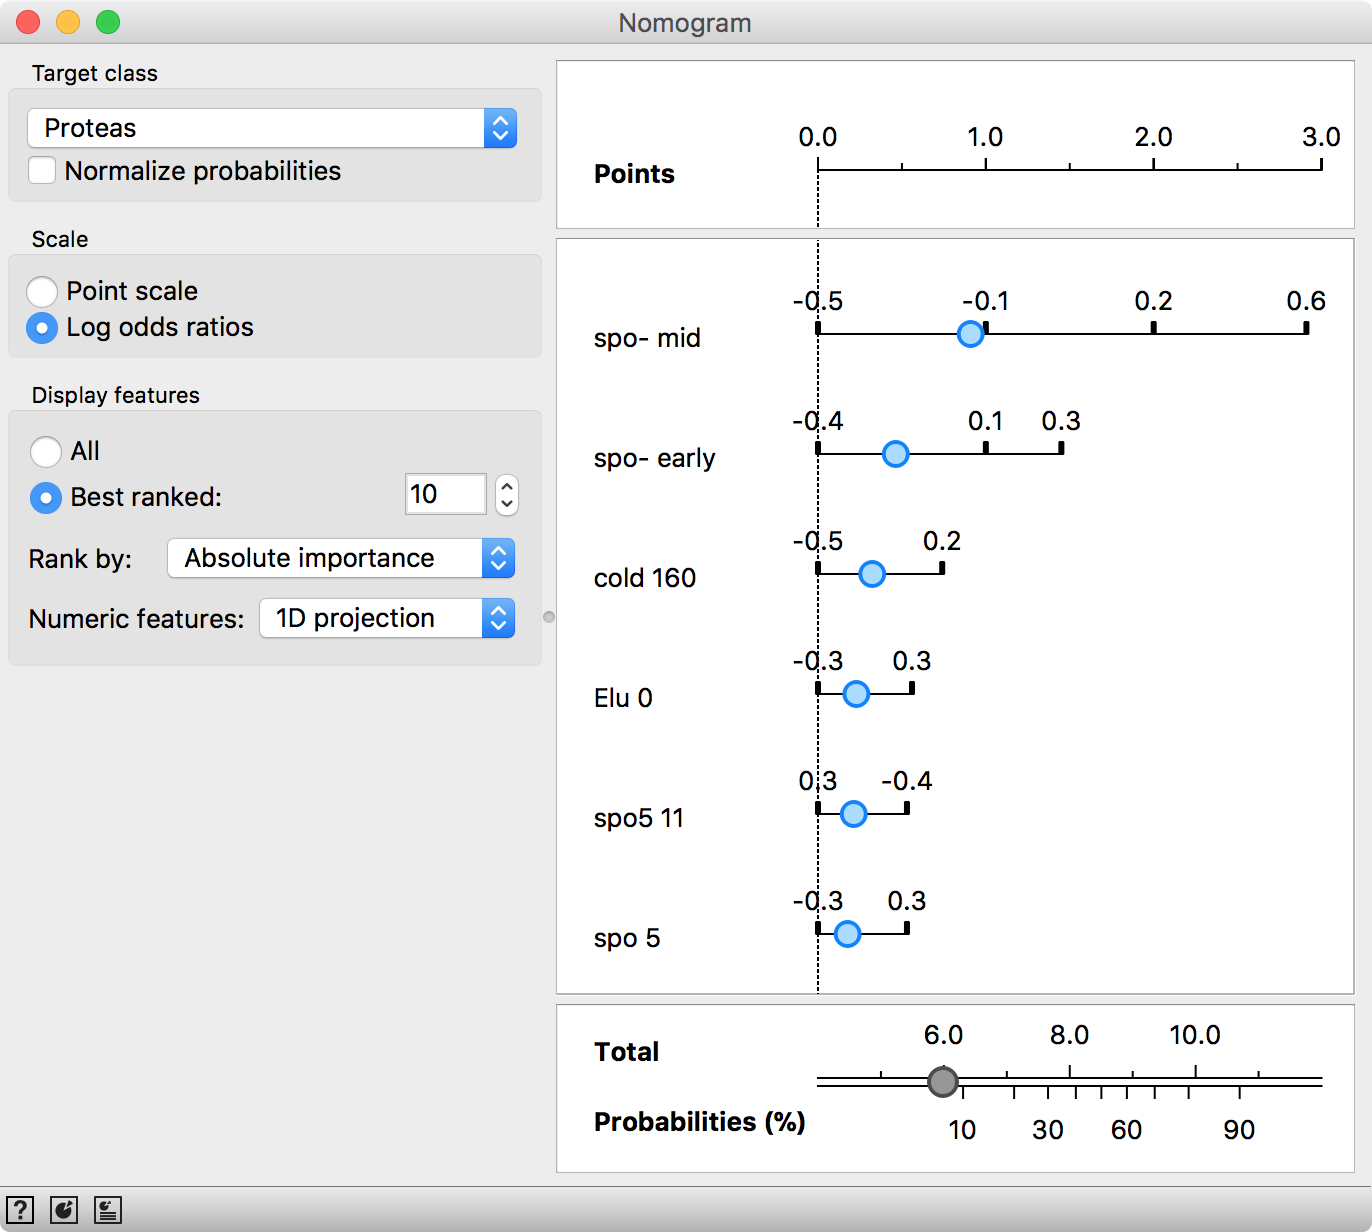
\includegraphics[scale=0.45]{nomogram.png}
    \caption{$\;$}
\end{wrapfigure}

V modelu logistične regresije ima vsaka spremenljivka svojo utež oz. pomembnost. Ko uporabimo model za napovedovanje novega primera, model pomnoži vrednosti spremenljivk z njihovimi utežmi, jih sešteje in nato pretvori v verjetnost. Končna vsota se pretvori v verjetnost z logistično funkcijo, ki jo vidimo na dnu nomograma.
